\section{Planteamiento del desarrollo del proyecto}
\rhostart{P}ara llevar a cabo el proyecto forKing fue necesario comprender cuál era el objetivo final al que se deseaba llegar razón por la cuál se ha decidido dividir el trabajo en dos fases: Gestión de memoria y planificación de procesos.


\subsection{Gestión de memoria}
En este punto fue necesario plantearse la manera en que se simularía la memoria dentro de forKing; ¿Se usaría memoria real a través de \texttt{Malloc()}? o tal vez ¿Podemos simular la memoria con un \textit{arreglo estático} donde asignar a cada uno de sus elementos una ``cantidad de memoria`` determinada?

Luego de investigar la gestión de memoria en diversos sistemas operativos se optó por hacer una implementación sencilla del sistema usado por \texttt{Linux}, el \textbf{BuddySystem} el cuál consiste en lo siguiente:
\begin{itemize}
    \item Se asume la memoria como un gran bloque de espacio disponible, supondremos un ejemplo con $2048$ bytes de memoria.
    \item Esta memoria construida tiene la capacidad de dividirse de manera \textit{binaria} recursivamente, lo que quiere decir, en el caso del ejemplo, que se pueden tener:
    \begin{itemize}
        \item Hasta $1$ bloque de $2048$ bytes
        \item Hasta $2$ bloques de $1024$ bytes
        \item Hasta $4$ bloques de $512$ bytes
        \item Hasta $8$ bloques de $256$ bytes
        \item Hasta $16$ bloques de $128$ bytes
        \item Hasta $32$ bloques de $64$ bytes
        \item Hasta $64$ bloques de $32$ bytes
        \item Etc$\dots$
    \end{itemize}
    \item Cuando un proceso requiere entrar en el BuddySystem se busca el bloque de memoria más cercano a la cantidad de memoria requerida (por encima) y asigna la memoria a dicho proceso, por ejemplo, si llegara un proceso que requiere de $500$ bytes de memoria, se asignaría un bloque de memoria de $512$ bytes, ya que este es el tamaño de bloque más cercano.
    \item Es aquí donde la división entra en juego. Si no existe un bloque de $512$ bytes de memoria, pero sí uno de $1024$ bytes, entonces este se dividirá en dos bloques de $512$ bytes, uno de los cuales será ocupado por el proceso, y el otro quedará libre para ser usado o fragmentado de ser necesario.
    \item Cuando un bloque se divide en dos más pequeños diremos que estos son \textit{Buddys} el uno del otro.
    \item En caso de que un proceso termine de usar un bloque de la memoria este queda libre. En este momento se evalúa si su \textit{Buddy} también está libre y, de ser así ambos se juntan generando un bloque más grande.
\end{itemize}

\begin{figure}[!ht]
    \centering
    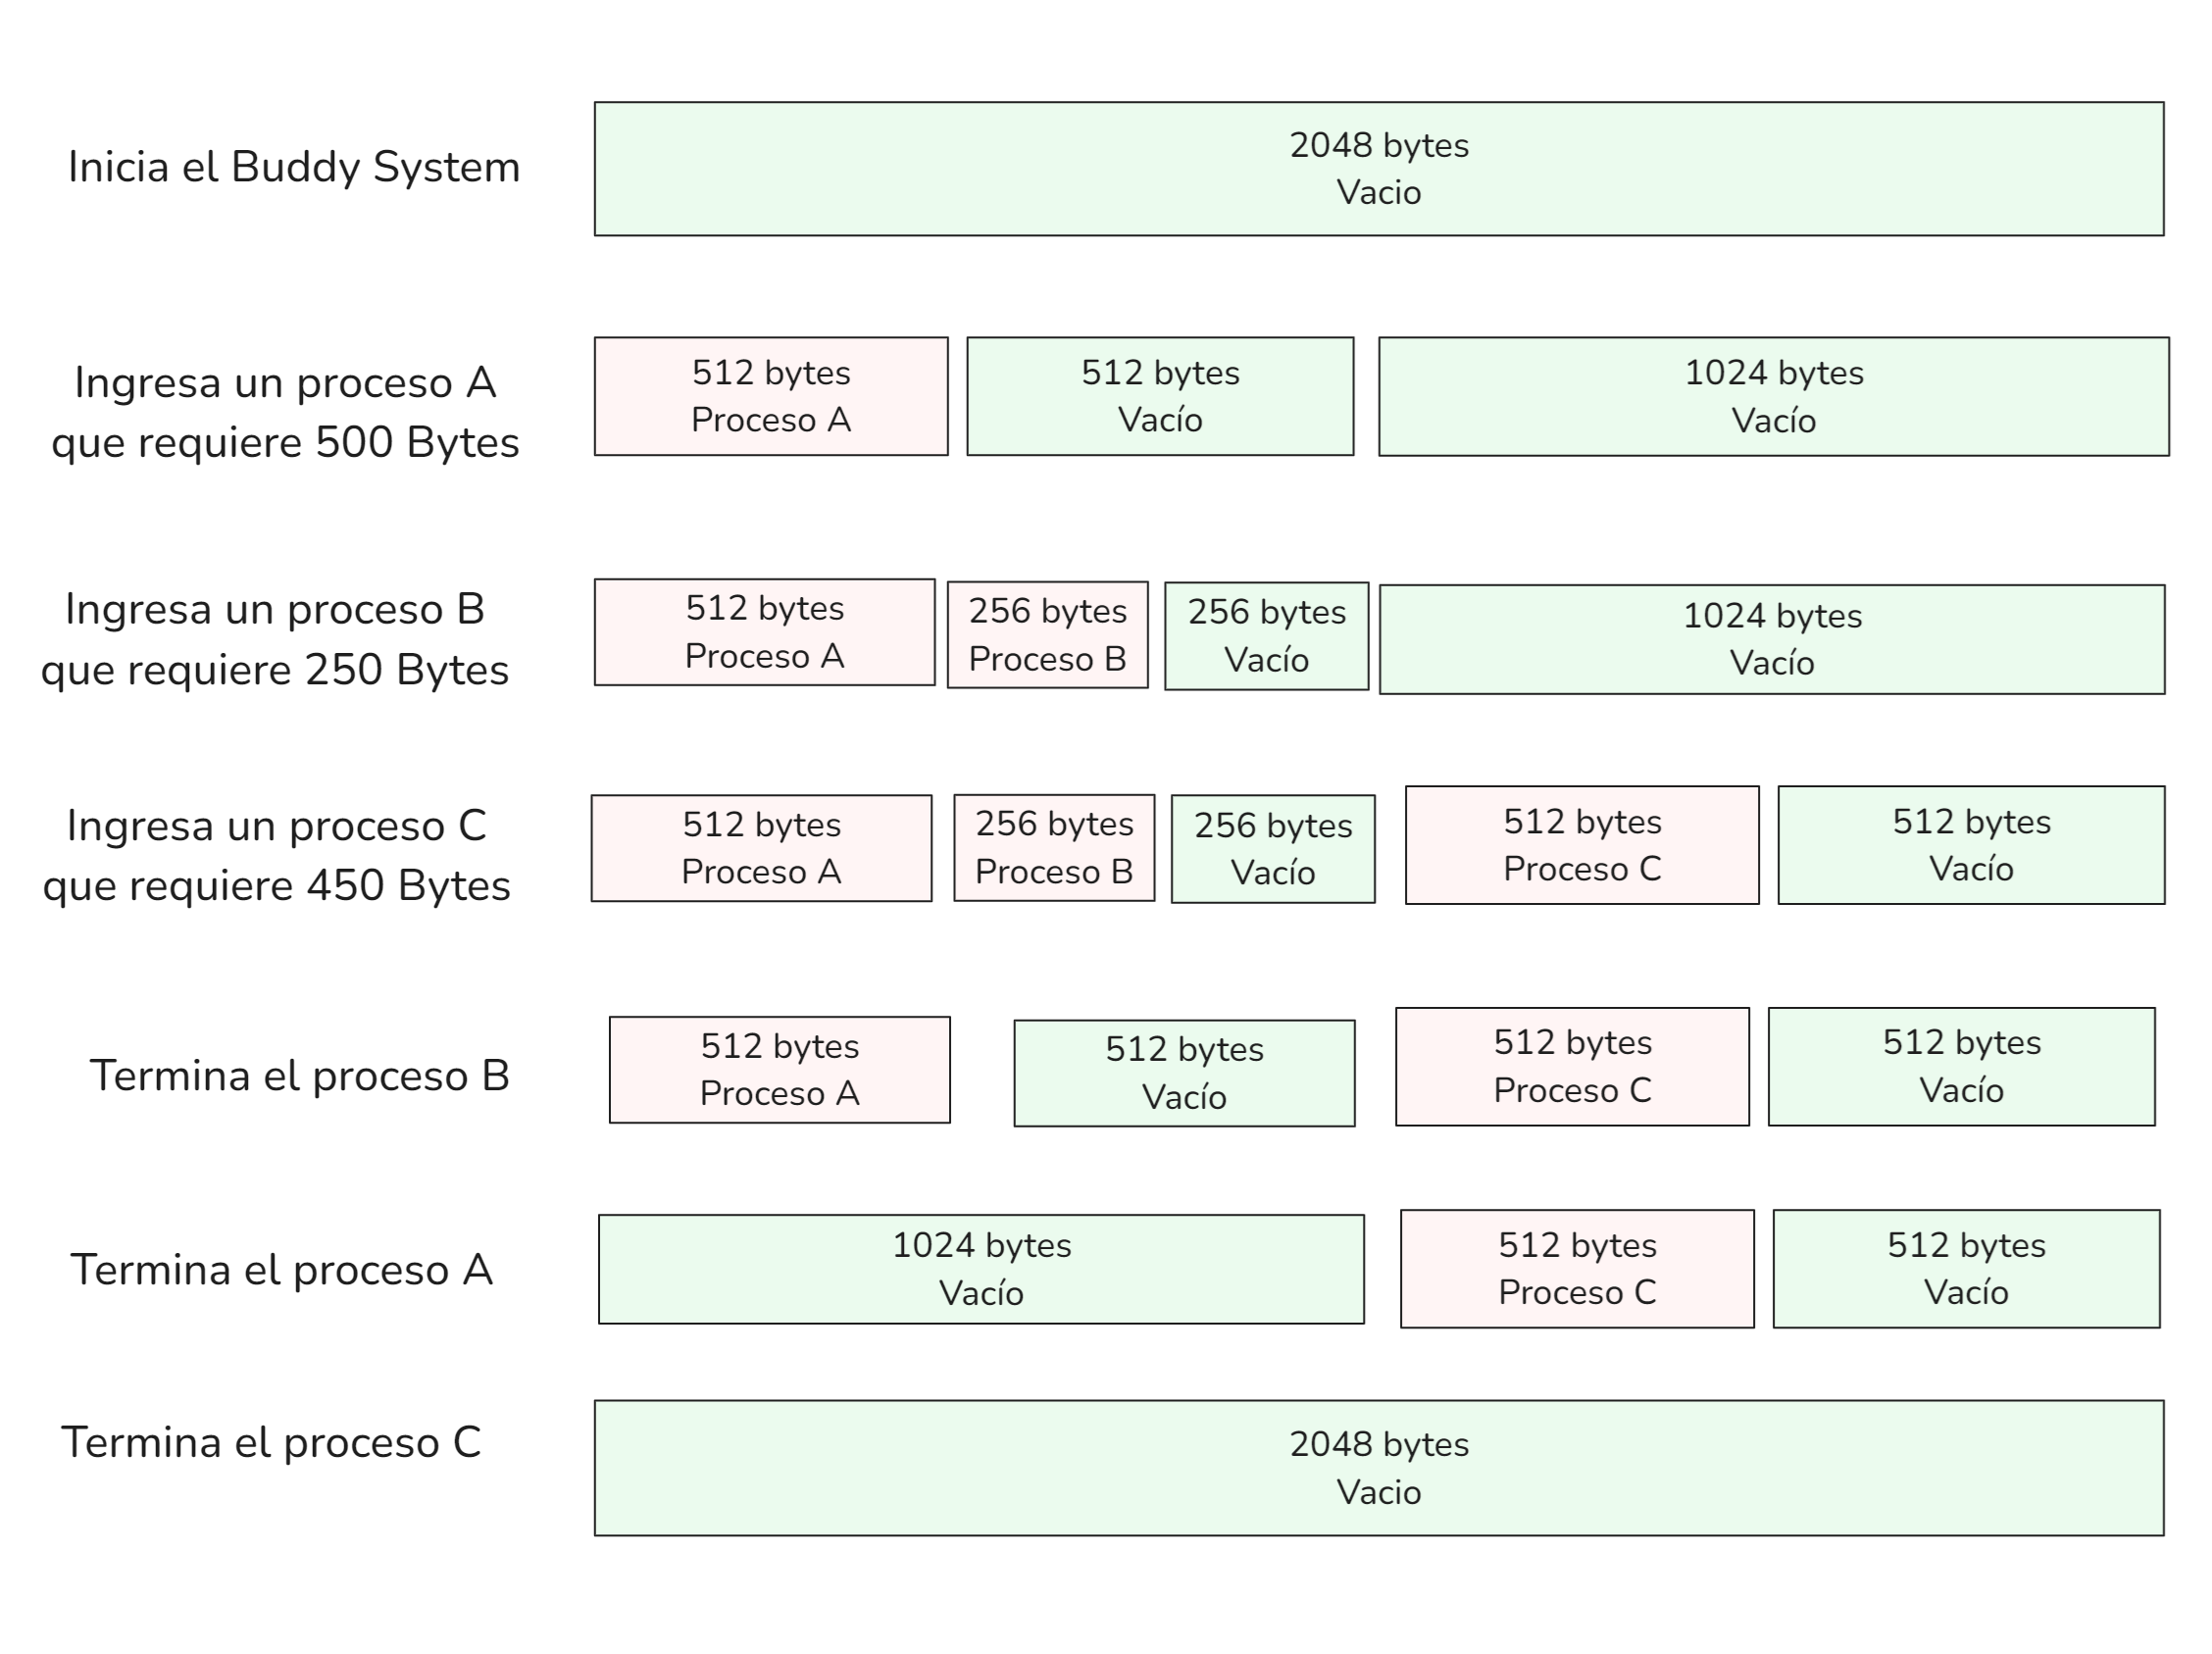
\includegraphics[width=0.8\textwidth]{src/figures/BuddyExample.png}
    \caption{Ejemplo de funcionamiento del buddySystem}\label{fig:buddyexample}
\end{figure}

\begin{note}
    Cada bloque dentro del \textit{BuddySystem} cuanta con una característica conocida como \textbf{Orden del bloque}, donde:

    Un bloque que no se puede dividir tendrá orden $0$ Y el orden irá ascendiendo hasta llegar al bloque más grande posible que tendrá el orden más alto posible.
\end{note}

¿Cuales son las ventajas de la utilización de un \textit{BuddySystem}? Principalmente que este sistema permite manejar de manera muy eficiente el fenómeno de la \textbf{Fragmentación de memoria} que ocurre que cuando procesos que requieren poca memoria terminan de ser procesados dejando partes muy pequeñas de la memoria vacías, lo que genera que, cuando un proceso que requiera de mucha memoria desee ser procesado, no encuentre un lugar lo suficientemente grande para ubicarse dentro de la memoria.

En la figura\ref{fig:buddyexample} se puede ver el comportamiento de un \textit{BuddySystem} de este tipo de manera gráfica.

\subsection{Manejo de procesos}
Una vez que ya tenemos una lista de procesos listos para su ejecución necesitamos de una manera eficiente para procesarlos. Una posible opción sería usar el algoritmo \texttt{FCFS} que consiste en atender a los procesos en el orden de llegada, sin embargo no es del todo eficiente, puesto que si llega un proceso que tarda $100s$ en ser ejecutado y detrás viene uno que tarda $10s$ este segundo deberá esperar demasiado tiempo para su ejecución.

Por esta razón surge el algoritmo \texttt{Shortest Job First} que consiste en atender a los procesos en el orden de su tiempo de ejecución (\texttt{burstTime}), sin embargo esto puede provocar que los procesos con mucho tiempo de ejecución no sean ejecutados nunca.

Para solucionar este último inconveniente aparece el algoritmo \texttt{Round Robin} donde todos los procesos sean parcialmente atendidos, dando como mínimo a cada uno $n$ ráfagas de CPU (\texttt{ticks}), donde $n$ es conocido como \texttt{quantum}. Así no existen procesos con tiempos de ejecución muy altos que no sean ejecutados.

En el presente proyecto se optó por el uso combinado de los algoritmos \texttt{Shortest Job First} y \texttt{Round Robin} en un modelo conocido como \textbf{algoritmo de colas multinivel} donde para un mismo Sistema Operativo se usan diversas colas que permiten un procesamiento eficiente de los recursos. El funcionamiento que se decidió dar al programa es el siguiente:

\begin{itemize}
    \item Un proceso cuyo \texttt{burstTime} es menor al \texttt{quantum} designado entra directamente a la cola \texttt{sjfQueue}.
    \item Un proceso cuyo \texttt{burstTime} es mayor o igual al \texttt{quantum} va a una cola que recibe el nombre de \texttt{rrQueue}.
    \item Si el \texttt{quantum} termina y el proceso sobre el que se trabajó tiene un tiempo restante menor al \texttt{quantum} va directamente a la \texttt{sjfQueue}.
    \item Por último la \texttt{sjfQueue} tiene más prioridad que la \texttt{rrQueue}, de forma que los procesos cortos se atienden primero y los largos se atienden mediante el \texttt{Round Robin}.
\end{itemize}

\subsection{Planificación general del proyecto}
Conociendo ya los conceptos usados en el proyecto resta solamente comentar cómo será la ejecución del programa, sin embargo antes se aclararán algunos conceptos adicionales propios del proyecto.
\begin{itemize}
    \item \textbf{ArrivalQueue}: Es una cola donde se almacenan los procesos que llegan a la simulación (Se asume que un proceso llega a la simulación si su \texttt{arrivalTime} coincide con la cantidad de \texttt{ticks} que han transcurrido desde que se inició el programa).
    \item \textbf{WaitingQueue}: Es una cola donde se almacenan los procesos que están esperando a ser procesados (Un proceso entra a esta cola si no existe memoria en el \texttt{BuddySystem} para este).
    \item \textbf{RRQueue}: Es una cola donde se almacenan los procesos que deben ser procesados por \texttt{Round Robin}.
    \item \textbf{SJFQueue}: Es una cola donde se almacenan los procesos que deben ser procesados por \texttt{Shortest Job First}.
    \item \textbf{BuddySystem}: Estructura de datos que representa el \textit{sistema} de buddies descrito anteriormente.
\end{itemize}

Con todas estas herramientas se describe el funcionamiento de \textit{forKing} en la figura \ref{fig:flowchart} donde se omiten comprobaciones varias de las colas para simplificar el diagrama.

\begin{figure}[!ht]
    \centering
    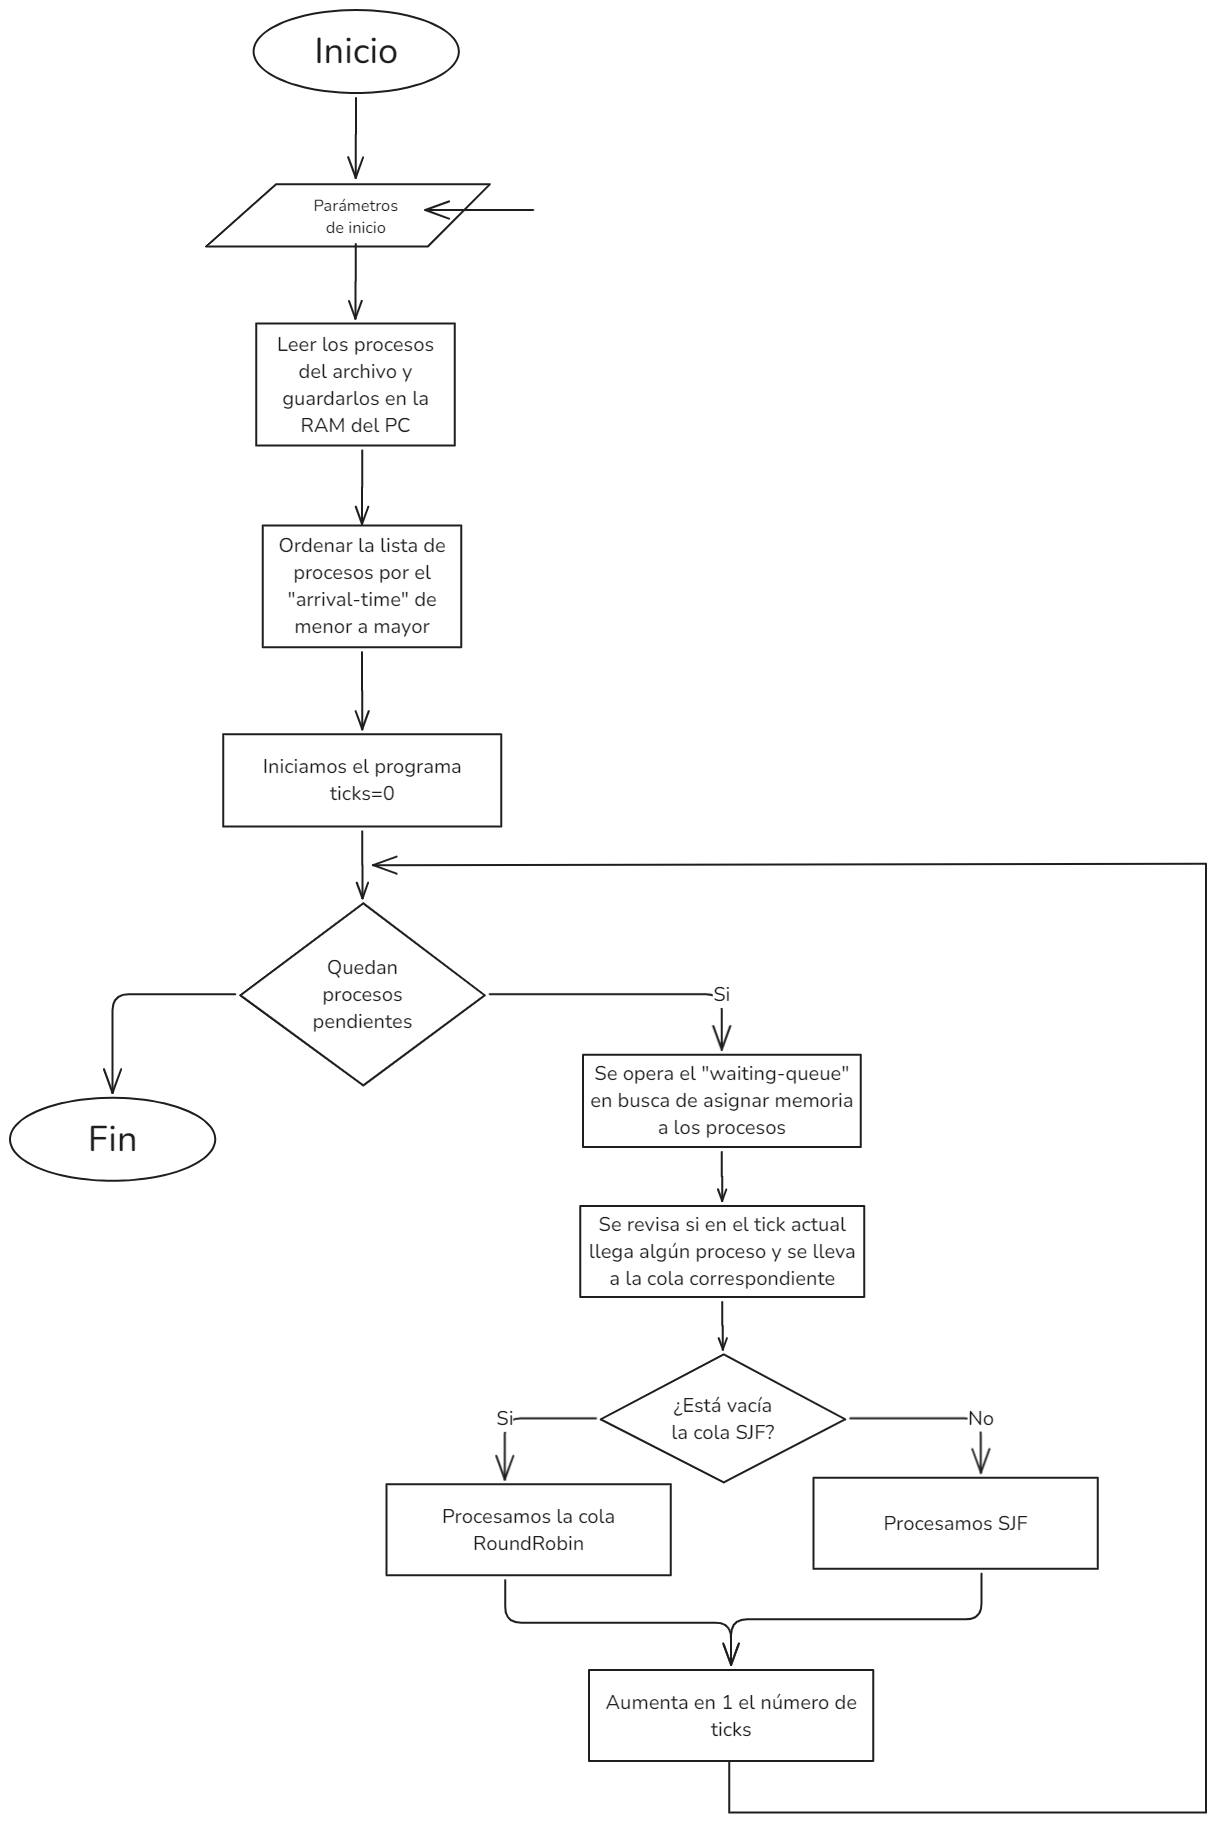
\includegraphics[height=12cm]{src/figures/Diagrama de flujo.png}
    \caption{Diagrama de flujo del desarrollo de forKing}\label{fig:flowchart}
\end{figure}

